%This is where you will assess the effectiveness of different thresholds and/or settings for the edge detection, and also establish which (if any) of your proposed filters and other methods actually improve performance, and how fast they are.

Edge detection is beneficial for Corner detector based on curvature properties \cite{Yung2008}, but not FAST and HARRIS. In this section, authors would like to explore the advantages of adaptive high and low thresholds in Canny edge detection introduced by MATLAB. In specific, Canny high threshold is determined by considering 30 percents highest values in edge image as edges while low threshold is 0.4 of the high one.


To appraise the effectiveness of adaptive high and low thresholds, two thermal images with high and low SNR are introduced followed by edge maps by applying divergent threshold values. The results are shown in Fig. \ref{fig:edgeprocessing}.


\begin{figure}
\centering
	\begin{subfigure}{0.49\columnwidth}
    \centering
    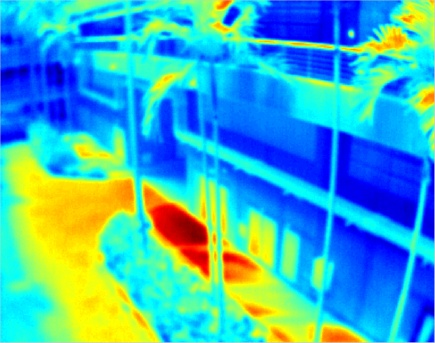
\includegraphics[width=1.00\textwidth]{media/V_E_highsnr.jpg}
	    \caption{}
		\label{fig:edgeprocessing_1}
  \end{subfigure}
	\begin{subfigure}{0.49\columnwidth}
    \centering
    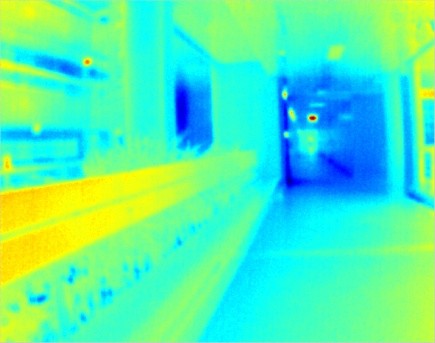
\includegraphics[width=1.00\textwidth]{media/V_E_lowsnr.jpg}
		\caption{}
		\label{fig:edgeprocessing_2}
  \end{subfigure} \vspace{10pt} \\ 
	\begin{subfigure}{0.49\columnwidth}
    \centering
    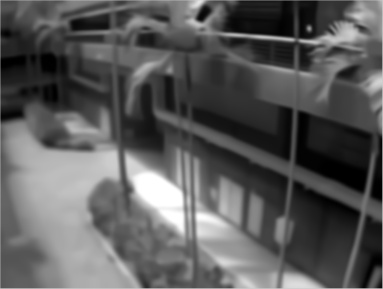
\includegraphics[width=1.00\textwidth]{media/V_E_highsnrori.jpg}
    	\caption{}
		\label{fig:edgeprocessing_3}
  \end{subfigure}
	\begin{subfigure}{0.49\columnwidth}
    \centering
    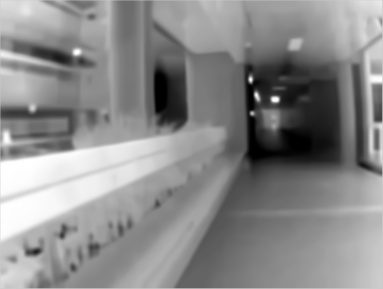
\includegraphics[width=1.00\textwidth]{media/V_E_lowsnrori.jpg}
		\caption{}
		\label{fig:edgeprocessing_4}
  \end{subfigure} \vspace{10pt} \\ 
	\begin{subfigure}{0.49\columnwidth}
    \centering
    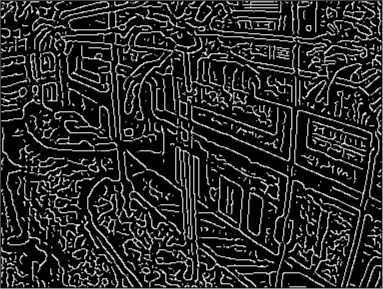
\includegraphics[width=1.00\textwidth]{media/V_E_highsnrlowcanny.jpg}
    	\caption{}
		\label{fig:edgeprocessing_5}
  \end{subfigure}
	\begin{subfigure}{0.49\columnwidth}
    \centering
    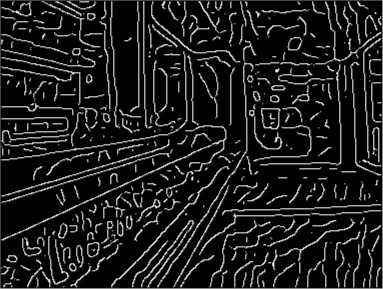
\includegraphics[width=1.00\textwidth]{media/V_E_lowsnrlowcanny.jpg}
		\caption{}
		\label{fig:edgeprocessing_6}
  \end{subfigure} \vspace{10pt} \\ 
	\begin{subfigure}{0.49\columnwidth}
    \centering
    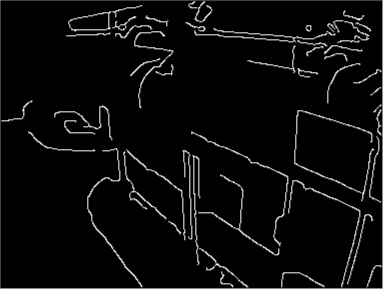
\includegraphics[width=1.00\textwidth]{media/V_E_highsnrhighcanny.jpg}
    	\caption{}
		\label{fig:edgeprocessing_7}
  \end{subfigure}
	\begin{subfigure}{0.49\columnwidth}
    \centering
    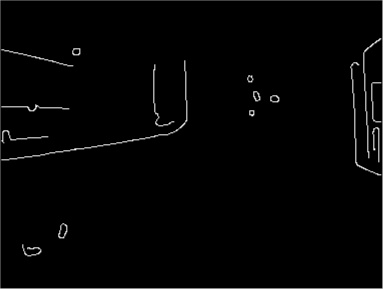
\includegraphics[width=1.00\textwidth]{media/V_E_lowsnrhighcanny.jpg}
		\caption{}
		\label{fig:edgeprocessing_8}
  \end{subfigure}  \vspace{10pt} \\  
  	\begin{subfigure}{0.49\columnwidth}
      \centering
      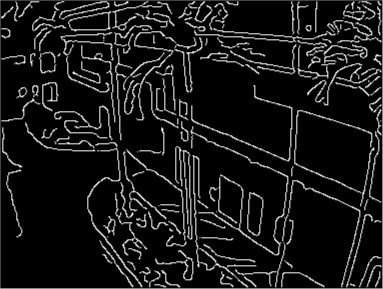
\includegraphics[width=1.00\textwidth]{media/V_E_highsnradapcanny.jpg}
      	\caption{}
  		\label{fig:edgeprocessing_9}
  \end{subfigure}
  	\begin{subfigure}{0.49\columnwidth}
      \centering
      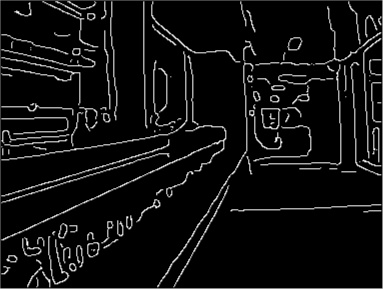
\includegraphics[width=1.00\textwidth]{media/V_E_lowsnradapcanny.jpg}
  		\caption{}
  		\label{fig:edgeprocessing_10}
    \end{subfigure}
  
\caption{Canny edge maps with different thresholds: (a,b) original outdoor high and low SNR frames, (c,d) gray-scale frames, (e,f) $L=0.004$ and $H=0.01$, (g,h) $L=0.16$ and $H=0.4$, (i) adaptive thresholds  $L=0.0625$ and $H=0.1563$, (j) adaptive thresholds $L=0.0313$ and $H=0.0781$}
\label{fig:edgeprocessing}
\end{figure}


